\section{Fouille de données textuelles}


\begin{frame}{Qu'est-ce que l'analyse textuelle ?}

    \onslide<1->
    \begin{block}{Définition}
        \medskip
        L'analyse textuelle, ou NLP, consiste à traiter et \textcolor{blue}{explorer} des textes pour en \textcolor{blue}{extraire} des informations utiles et \textcolor{blue}{comprendre} leur contenu.

        C'est une extension du data mining à des \textcolor{red}{corpus} de textes
    \end{block}
    
    \onslide<2->
    \begin{block}{Pourquoi ?}
        \medskip
        Elle permet d'\textcolor{blue}{automatiser} la compréhension des textes en identifiant des tendances, des sentiments, ou des thèmes.
    \end{block}

\end{frame}

\begin{frame}{Information utile ?}

    \onslide<1-> \textsc{Quels sont les mots les plus représentés ?}
    \medskip

    \onslide<2-> \textsc{Quels sont les sujets abordés ?}
    \medskip
    
    \onslide<3-> \textsc{Quels sont les concepts clés et les relations entre eux ?}
    \medskip
    
    \onslide<4-> \textsc{Quels sont les phrases ou les paragraphes spécifiques au sujet du texte ?}
    \medskip

    \onslide<5-> \textsc{Quelle est la structure logique d'un texte ?}

\end{frame}



\begin{frame}{Exemple 1 : fréquence des mots}
    Calcul du \textbf{nombre d'occurrence} de chaque mot dans un texte.
    \bigskip
    \begin{columns}
        \begin{column}{.48\textwidth}
            \centering
            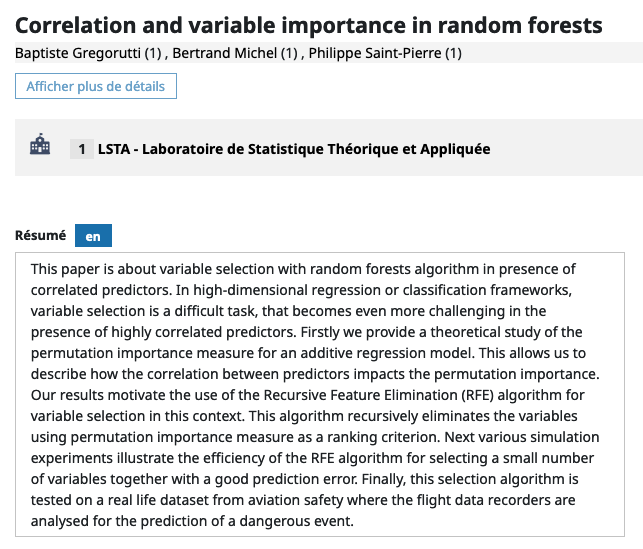
\includegraphics[width=\textwidth]{img/example-text.png}
        \end{column}
        \begin{column}{.48\textwidth}
            \centering
            \begin{tabular}{c|c} 
                \hline
                \textbf{Mot} & \textbf{Fréquence} \\ 
                \hline
                Variable & 5 \\
                Selection & 4 \\
                Algorithm & 3 \\
                Correlated & 3 \\
                Predictors & 2 \\
                Regression & 2 \\
                Importance & 2 \\
                \hline
            \end{tabular}
        \end{column}
        \end{columns}
\end{frame}

\begin{frame}{Exemple 2 : mots clés}
    Extraction des \textbf{mots clés} $\rightarrow$ identifier les \textcolor{red}{idées} principales
    \bigskip

    \begin{columns}
    \begin{column}{.48\textwidth}
        \centering
        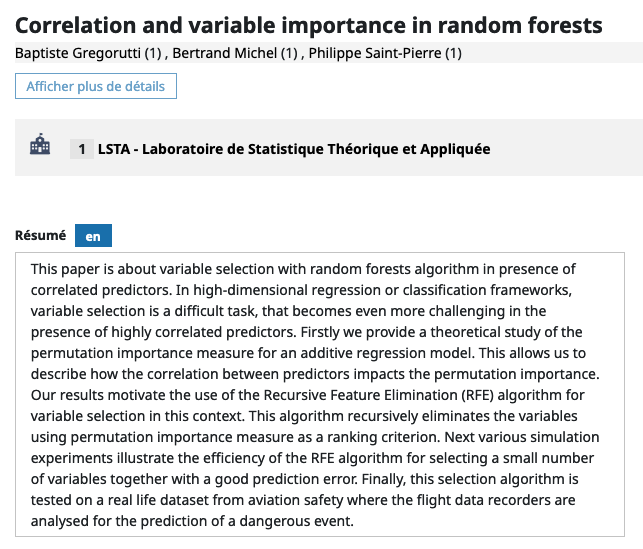
\includegraphics[width=\textwidth]{img/example-text.png}
    \end{column}
    \begin{column}{.48\textwidth}
        \centering
        
\includegraphics[width=\textwidth]{img/word-cloud.png}
    \end{column}
    \end{columns}
\end{frame}


\begin{frame}{Exemple 3 : entités nommées}
    Extraction des \textbf{entités nommées} $\rightarrow$ identifier les personnes, lieux, organisations, dates, etc.
    \bigskip

    \begin{columns}
    \begin{column}{.33\textwidth}
        \centering
        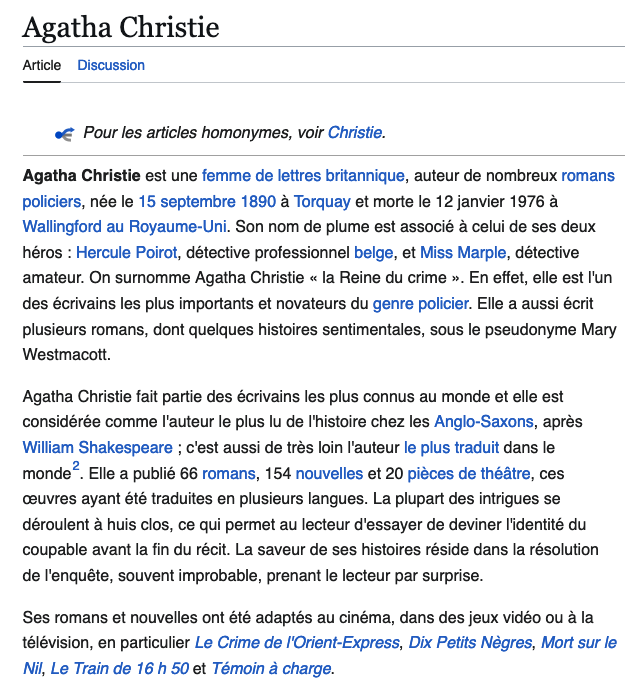
\includegraphics[width=\textwidth]{img/agatha-wiki.png}
    \end{column}
    \begin{column}{.66\textwidth}
        {\footnotesize
        \textbf{Personnes} : Agatha Christie, Hercule Poirot, Miss Marple, William Shakespeare \\
        \medskip
        \textbf{Lieux} : Torquay, Wallingford, Royaume-Uni \\
        \medskip
        \textbf{Dates} : 15 septembre 1890, 12 janvier 1976 \\
        \medskip
        \textbf{Genres et styles} : Roman policier, théâtre \\
        \medskip
        \textbf{Médias} : Cinéma, jeux vidéo}
    \end{column}
    \end{columns}
\end{frame}




\begin{frame}{Exemple 4 : analyse de sentiments}
    L'analyse de sentiments consiste à identifier le ton d'un texte
    \bigskip

    \begin{overprint}
        \onslide<2>
        \begin{columns}
            \begin{column}{.48\textwidth}
                \centering
                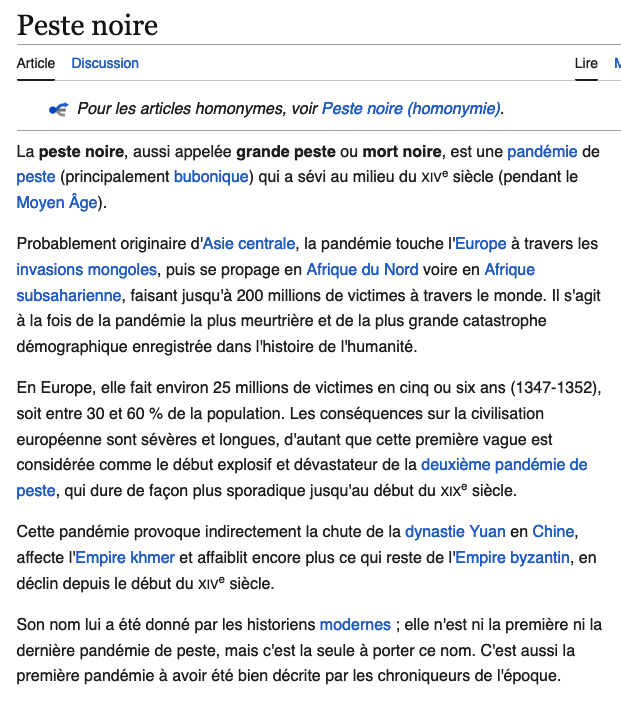
\includegraphics[width=\textwidth]{img/peste.png}
            \end{column}
            \begin{column}{.48\textwidth}
                \centering
                
\includegraphics[width=.4\textwidth]{img/negative.png}
            \end{column}
        \end{columns}

        \onslide<1>
        \begin{columns}
            \begin{column}{.48\textwidth}
                \centering
                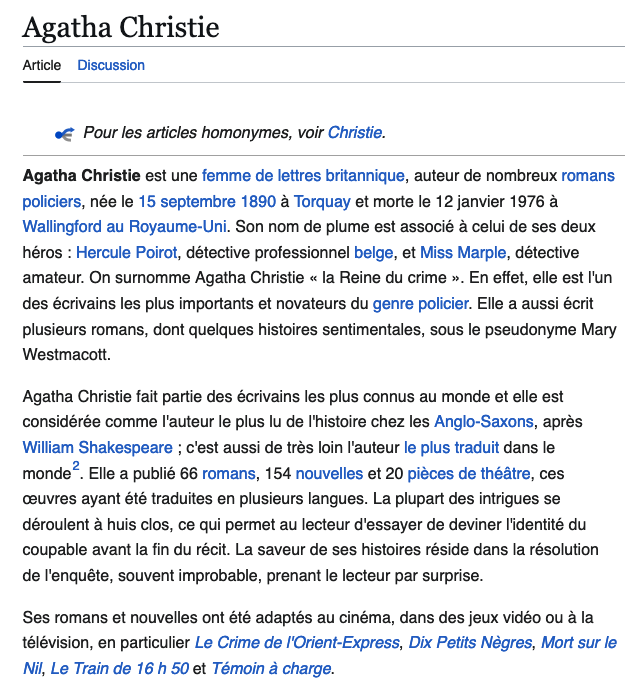
\includegraphics[width=\textwidth]{img/agatha-wiki.png}
            \end{column}
            \begin{column}{.48\textwidth}
                \centering
                
\includegraphics[width=.4\textwidth]{img/positive.png}
            \end{column}
        \end{columns}

        \onslide<3>
        \begin{columns}
            \begin{column}{.48\textwidth}
                \centering
                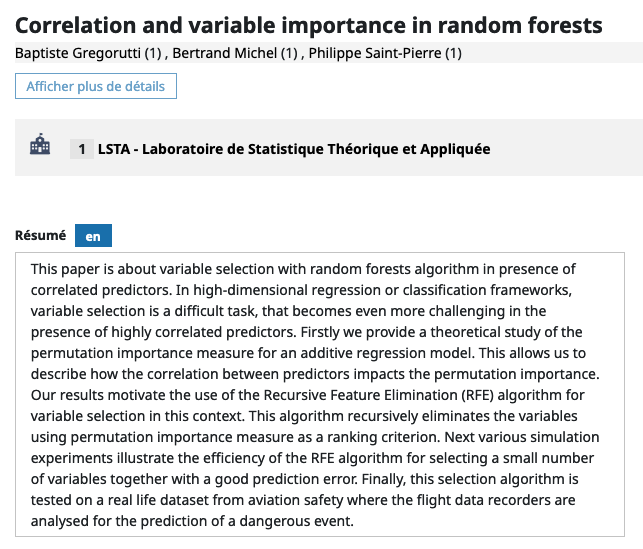
\includegraphics[width=\textwidth]{img/example-text.png}
            \end{column}
            \begin{column}{.48\textwidth}
                \centering
                
\includegraphics[width=.4\textwidth]{img/neutral.png}
            \end{column}
        \end{columns}

    \end{overprint}


\end{frame}



\begin{frame}{Exemple 5 : segmentation de texte}
    Consiste à identifier la structure d'un document

    \begin{columns}
        \begin{column}{.4\textwidth}
        \end{column}
        \begin{column}{.6\textwidth}
            \centering
            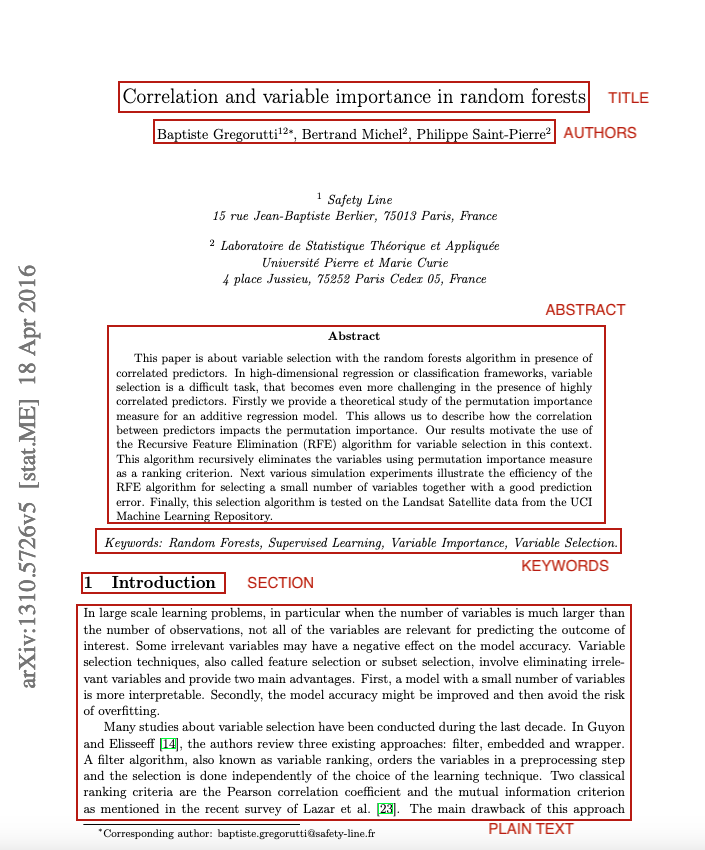
\includegraphics[width=\textwidth]{img/segmentation-example.png}
        \end{column}
    \end{columns}

\end{frame}

\section{Importance du contexte}

\begin{frame}{Importance du contexte}
    \fbox{
        \parbox{\textwidth}{
            La prise en compte du contexte est la capacité à \textbf{interpréter correctement le sens des mots ou des phrases}, et ainsi à améliorer la précision des analyses
        }
    }

    \bigskip
    
    \centering
    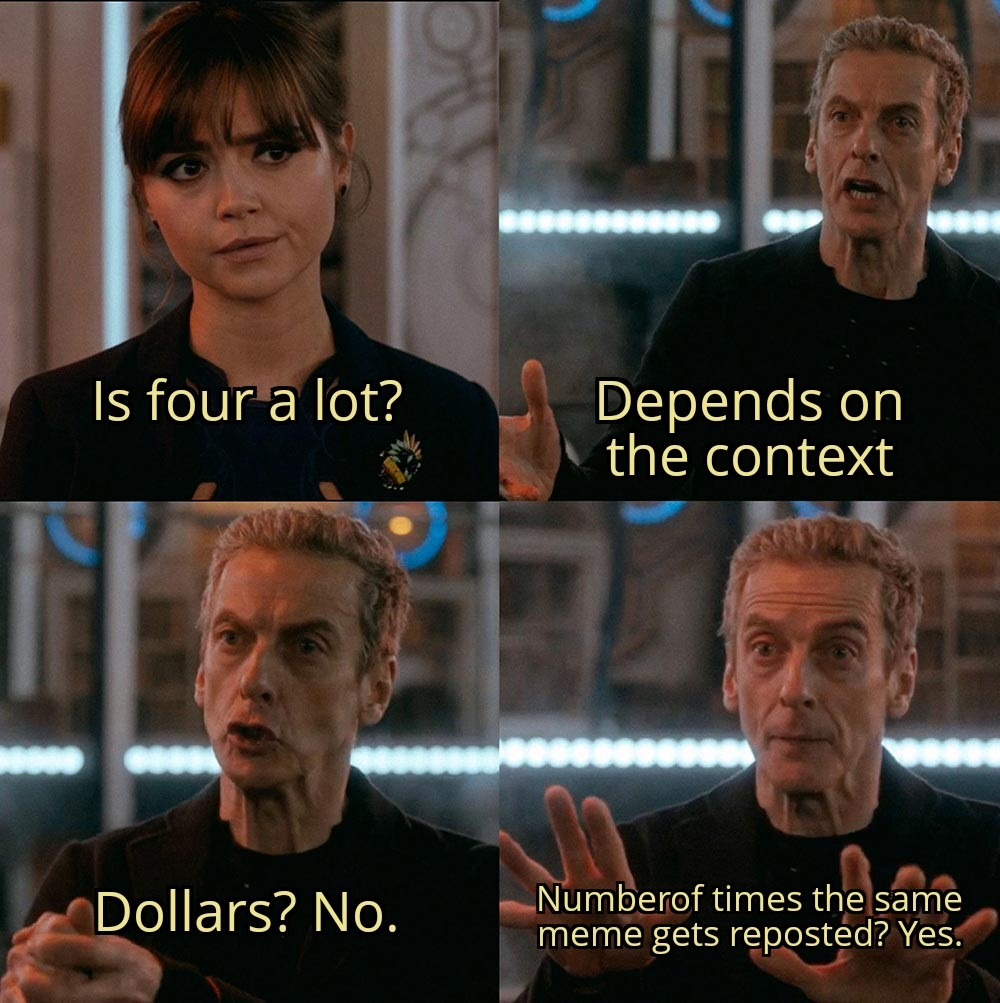
\includegraphics[width=.4\textwidth]{img/context.jpeg}

\end{frame}

\begin{frame}{Importance du contexte}
\footnotesize{
        \onslide<1->
        \begin{block}{Ambiguité lexicale (polysémie)}
            \smallskip
            Un mot peut avoir plusieurs sens\\Ex : bureau, affection, légende
        \end{block}

        \onslide<2->
        \begin{block}{Relations sémantiques}
            \smallskip
            Le sens d'un mot peut être influencé par les mots qui l'entourent\\Ex : banque de prêts vs banque d'organes
        \end{block}

        \onslide<3->
        \begin{block}{Ambiguité dans les entités}
            \smallskip
            Certaines entités nécessitent un contexte pour être correctement identifiées\\Ex : Apple vs apple ou bien Paris vs paris
        \end{block}

        \onslide<4->
        \begin{block}{Compréhension du sens global}
            \smallskip
            Les outils modernes ont besoin du contexte pour mieux comprendre le sens global d'une phrase
        \end{block}
 }  
\end{frame}



\section{Quelques concepts techniques}

\begin{frame}{Stop Words}

    \begin{block}{Définition}
        \smallskip
        Mots fréquents et \textcolor{red}{peu significatifs} dans une langue :\\\texttt{"et"}, \texttt{"le"}, \texttt{"de"}, etc.
    \end{block}

    \bigskip

    \begin{block}{Objectif}
        \smallskip
       Les \textcolor{red}{exclure} pour se concentrer sur le contenu pertinent.
    \end{block}
\end{frame}

\begin{frame}{Tokenization}
    \begin{block}{Qu'est-ce qu'un token ?}
        \smallskip
        \begin{itemize}
            \item Un \textbf{mot}\\
            {\footnotesize \texttt{"Bonjour. Comment ça va ?"} $\rightarrow$ [\texttt{"Bonjour"}, \texttt{"Comment"}, \texttt{"ça"}, \texttt{"va"}]}
            \item Une \textbf{phrase}\\
            {\footnotesize \texttt{"Bonjour. Comment ça va ?"} $\rightarrow$ [\texttt{"Bonjour."}, \texttt{"Comment ça va ?"}]}
            \item Un \textbf{sous-mot}\\
            {\footnotesize \texttt{"impossible"} $\rightarrow$ [\texttt{"im"}, \texttt{"possible"}]}
        \end{itemize}
        
    \end{block}
    
    \bigskip
    
    \begin{block}{Objectif de la tokenization}
        \smallskip
        Diviser un texte en \textbf{tokens} pour en faciliter l'analyse
    \end{block}
\end{frame}



\begin{frame}{Tokenization}
    \begin{block}{Qu'est-ce qu'un token ?}
        \smallskip
        \begin{itemize}
            \item Un \textbf{mot}\\
            {\footnotesize \texttt{"Bonjour. Comment ça va ?"} $\rightarrow$ [1, 2, 3, 4]}
            \item Une \textbf{phrase}\\
            {\footnotesize \texttt{"Bonjour. Comment ça va ?"} $\rightarrow$ [5, 6]}
            \item Un \textbf{sous-mot}\\
            {\footnotesize \texttt{"impossible"} $\rightarrow$ [7, 8]}
        \end{itemize}
        
    \end{block}
    
    \bigskip
    
    \begin{block}{Objectif de la tokenization}
        \smallskip
        Diviser un texte en \textbf{tokens} pour en faciliter l'analyse
    \end{block}
\end{frame}



\begin{frame}{Lemmatisation}

    \begin{block}{Qu'est-ce qu'un lemme ?}
        \smallskip
        La forme canonique d'un mot.
    \end{block}

    \bigskip

    \begin{block}{Objectif de la lemmatisation}
        \smallskip
        Réduire les mots à leur \textcolor{blue}{forme canonique}\\
        Ex : \texttt{mangeait} $\rightarrow$ \texttt{manger}

        A ne pas confondre avec la racinisation (stemming)
    \end{block}

\end{frame}

\begin{frame}{Plongement lexical}
    
    \begin{block}{Définition}
        \smallskip
        Le plongement lexical, ou plongement sémantique, vise à représenter les \textcolor{red}{mots} sous forme de \textcolor{red}{vecteurs}.
    \end{block}

    \bigskip

    \begin{overprint}
        \onslide<1>
        \centering
        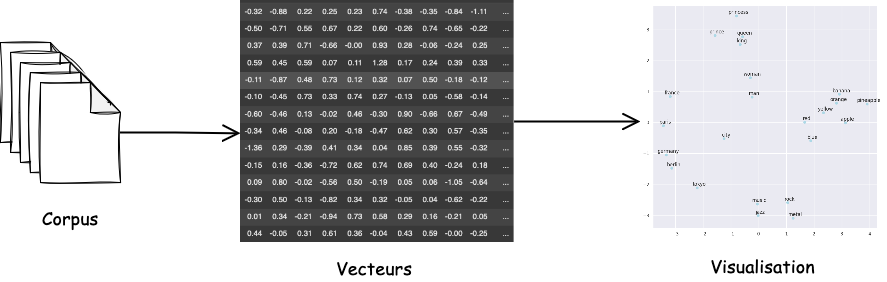
\includegraphics[width=\textwidth]{img/embedding-vizu.png}

        \onslide<2>
        \begin{block}{Pourquoi ?}
            \smallskip
            Pour utiliser les outils statistiques (visualisation et modélisation) tout simplement !
        \end{block}

    \end{overprint}
\end{frame}

\begin{frame}{Plongement lexical}
    \centering
    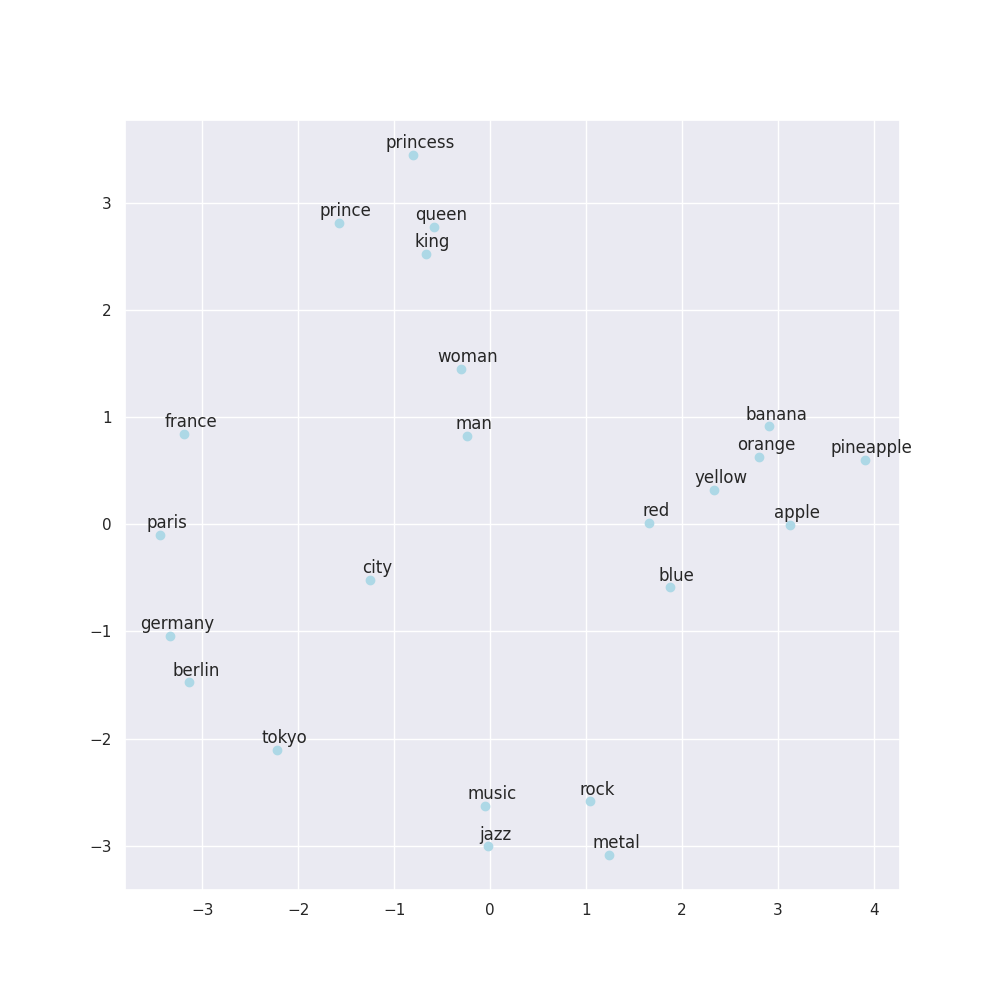
\includegraphics[width=.8\textwidth]{img/glove.png}
\end{frame}






\section{Cas d'usage}

\begin{frame}{Cas d'usage}
\footnotesize{
    \onslide<1->
    \begin{block}{Marketing}
        \smallskip
        Marketing ciblé, publicité personnalisée, support client
    \end{block}

    \bigskip

    \onslide<2->
    \begin{block}{Recherche historique}
        \smallskip
            Analyse de corpus historique pour aider la recherche
    \end{block}

    \bigskip

    \onslide<3->
    \begin{block}{Bases de données documentaires}
        \smallskip
        Indexer, structurer une base de données et moteurs de recherche
        Classification de documents, dé-doublonnage
    \end{block}
}
\end{frame}
